\documentclass[a4paper,11pt]{article}
\usepackage{graphicx}
\usepackage[utf8]{inputenc}
\usepackage{hyperref}
\usepackage{placeins}
\usepackage{minted}


\hypersetup{
    colorlinks=true,
    linkcolor=blue,
    filecolor=black,      
    urlcolor=blue,
    citecolor=black,
}
\begin{document}

\title{
    \textbf{Sorting Report.}
}
\author{Adrian Jonsson Sjödin}
\date{Fall 2022}

\maketitle

\section*{Introduction}
The task in this assignment was to explore some different sorting algorithms to gain a
better understanding how different implementations can affect the time it takes to sort
a large array.
\section*{Task}
Implement the three following sorting algorithms: Selection sort, Insert sort and Merge
sort. For each of the algorithms explain the run time as a function of the size of the
array and state their time complexity using Big O notation. Lastly do some benchmark and
compare how the different algorithms compares to each other.

\section*{Method \& Theory}
The Selection Sort algorithm was the first to be implemented and is quite straight forward.
It takes the first element and then looks through the array to see if there's an element
smaller than it. When it has looked through the whole array it swaps the first element with
the found minimum element and then goes on to the next element and repeat the process
until the end of the array has been reached. This means that it will have a time complexity
of $\mathcal{O}(n^2)$ since it will have to take one element at a time (out of $n$ elements)
and look through an array of size $n$ to see if there's a smaller element $n-1$ times.

The second algorithm to be implemented was the Insertion Sort algorithm which is slightly
more complicated to implement. Instead of looking through the array from start to end after the smallest element, this algorithm
compare the element it is looking at with the previous element and its previous element until it finds the spot where it fits in
the array. In best case if the array is already sorted so should this algorithm give us a time complexity of $\mathcal{O}(n-1)=\mathcal{O}(n)$,
since it then only need to go through the array once doing $n-1$ comparisons checking that every value is larger than its predecessor.
On average though it should have a time complexity of $\mathcal{O}(n^2)$ since it will have to go through an array of size $n$ and for each element $i\in n$
do up to $i-1$ comparisons for $i \to n$.

Lastly we implement the Merge Sort algorithm which was by far the hardest to implement because of its recursive nature. This algorithm works by first splitting
an array in halves recursively until further division becomes impossible. After this step we start merging the elements back together again based on comparison
of size of the elements. We compare the elements for each sublist and then combine them together into another list in a sorted manner. Figure \ref{fig:mergeSort}
visualizes this in a good way.
\begin{figure}
    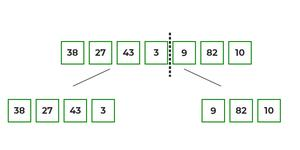
\includegraphics[width =.5\textwidth]{mergesort1.jpg}
    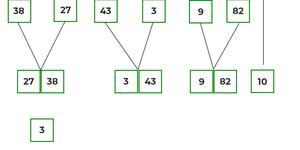
\includegraphics[width =.5\textwidth]{mergesort3.jpg}
    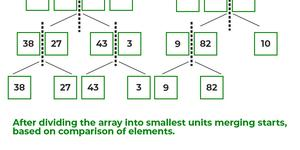
\includegraphics[width =.5\textwidth]{mergesort2.jpg}
    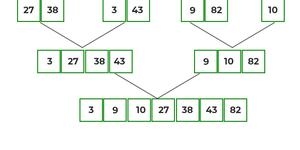
\includegraphics[width =.5\textwidth]{mergesort4.jpg}
    \caption{Merge Sort. Read top down, left to right. \href{https://www.geeksforgeeks.org/merge-sort/}{Picture source}}
    \label{fig:mergeSort}
\end{figure}
I haven't included the code fort the recursive call here in the report since the teacher already went through that part during his lecture, and thus would be
redundant to show again, but for those interested all the code can be found here: \href{https://github.com/adrian-jonsson-sjoedin/ID1021-AlgoData/blob/main/Tasks/Sorting/src}{GitHub}

\section*{Result}
Bellow you can see the data from the benchmarked run for the different algorithms as well as plots over how the time execution increase with the array size. The 
benchmark is the minimum average time it took to sort an array of size n over 1000 loops.
\begin{table}[h!]
    \begin{center}
        \begin{tabular}{|c|c|c|c|c|c|}
            \hline
            \textbf{Array size} & \textbf{Select} & \textbf{Insert} & \textbf{$\frac{select}{insert}$} & \textbf{Merge} & \textbf{$\frac{insert}{merge}$} \\
            \hline
            100                 & 3.80            & 1.34            & 2.84                             & 2.76           & 0.48                            \\
            200                 & 11.0            & 4.11            & 2.68                             & 5.21           & 0.79                            \\
            400                 & 43.3            & 14.3            & 3.03                             & 9.61           & 1.49                            \\
            800                 & 165.1           & 54.8            & 3.01                             & 31.7           & 1.73                            \\
            1,600               & 603.3           & 214.9           & 2.81                             & 90.6           & 2.37                            \\
            3,200               & 2,439.2         & 855.9           & 2.85                             & 243.2          & 3.52                            \\
            6,400               & 9,642.7         & 3,375.8         & 2.86                             & 513.3          & 6.58                            \\
            12,800              & 45,481.7        & 16,778.1        & 2.71                             & 1247.0         & 13.45                           \\
            \hline
        \end{tabular}
        \caption{Benchmark for the different sorting algorithm. Time in $\mu s$}
        \label{tab:benchmark}
    \end{center}
\end{table}

\begin{figure}[h!]
    \centering
    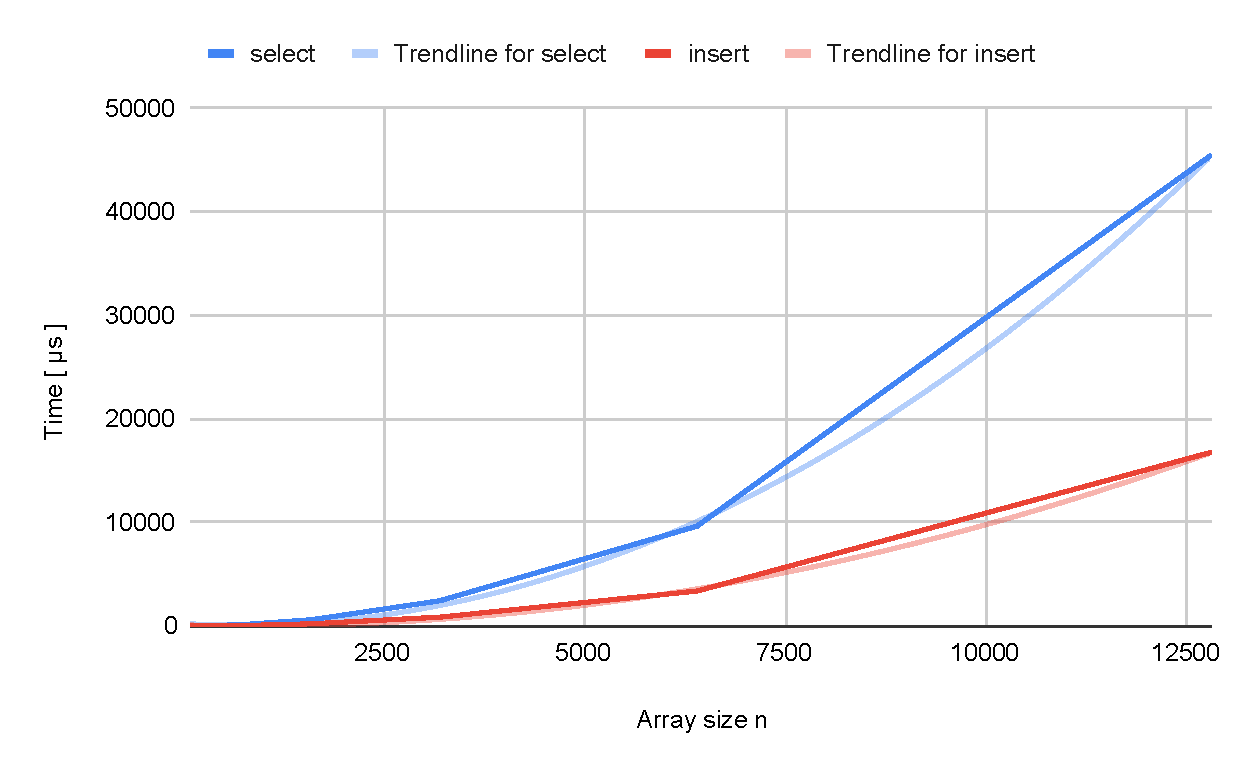
\includegraphics[width=.8\textwidth]{Select and Insert Sort.pdf}
    \caption{Select vs. Insert Sort}
    \label{fig:selectInsert}
\end{figure}

\begin{figure}[h!]
    \centering
    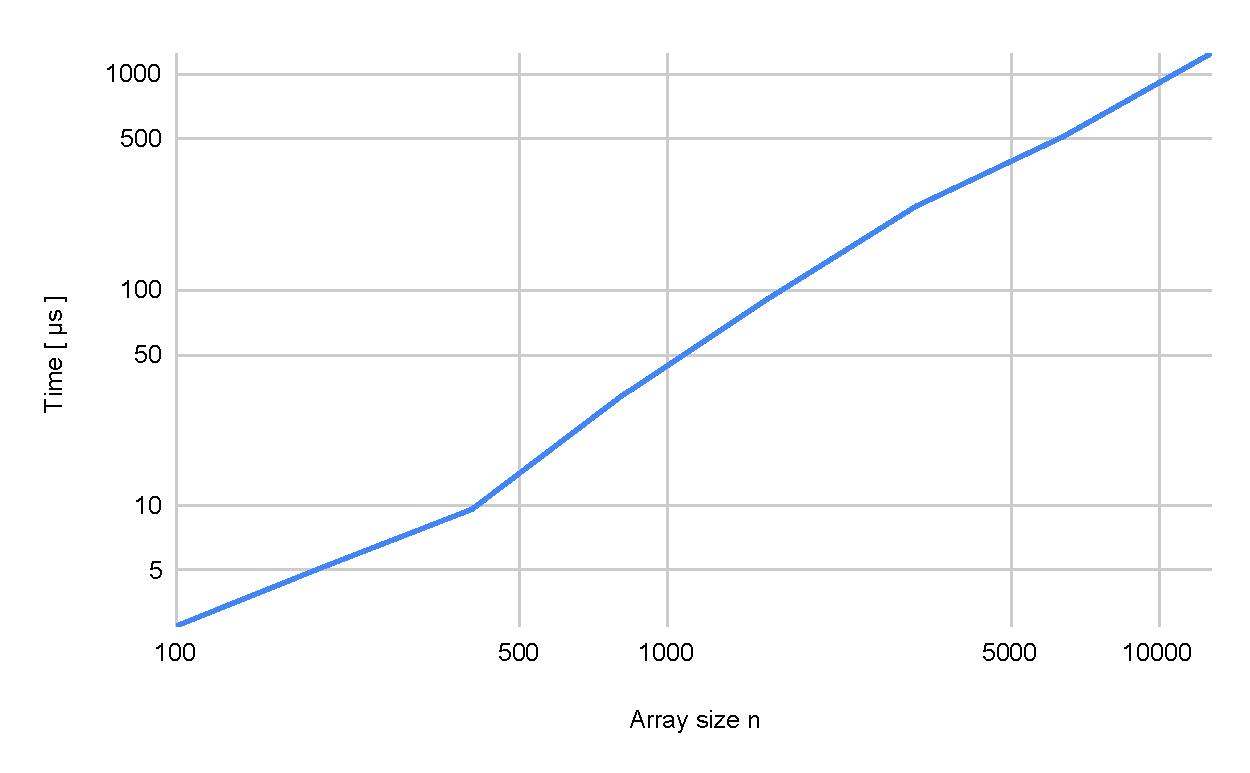
\includegraphics[width=.8\textwidth]{Merge Sort.pdf}
    \caption{Merge Sort}
    \label{fig:merge}
\end{figure}
\section*{Discussion}




\end{document}
